% begin module inverse-function-graph
\begin{frame}
\begin{tabular}{cc}
\psset{xunit=1cm, yunit=1cm}
\begin{pspicture}(-5, -5)(5,5) 
\psframe*[linecolor=white](-5,-5)(5,5) 
\psaxes[ticks=none, labels=none]{<->}(0,0)(-1.5,-1.5)(3,3)

\uncover<6->{
\psline(2.5, 1)(1, 2.5)
\psline(1.85, 1.65)(1.95, 1.75)(1.85, 1.85)
\psline(1.85, 1.85)(1.75, 1.95)(1.65, 1.85)

\psline(1.9875, 1.3125)(2.1875, 1.5125)
\psline(2.0625, 1.2375)(2.2625, 1.4375)
\psline(1.3125, 1.9875)(1.5125, 2.1875)
\psline(1.2375, 2.0625)(1.4375, 2.2625)

\psline[linecolor=blue](-1.35, -1.35)(2.8,2.8)
\rput[l](-1, -1.2){\footnotesize $y=x$}
}
\psFullDot{2.5}{1}
\rput[lt](2.6, 1.1){\footnotesize $(a,b)$}
\uncover<5->{
\psFullDot{1}{2.5}
\rput[rb](0.9, 2.6){\footnotesize $(b,a)$}
}
\end{pspicture}
%\ \only<handout:0| -4>{%
%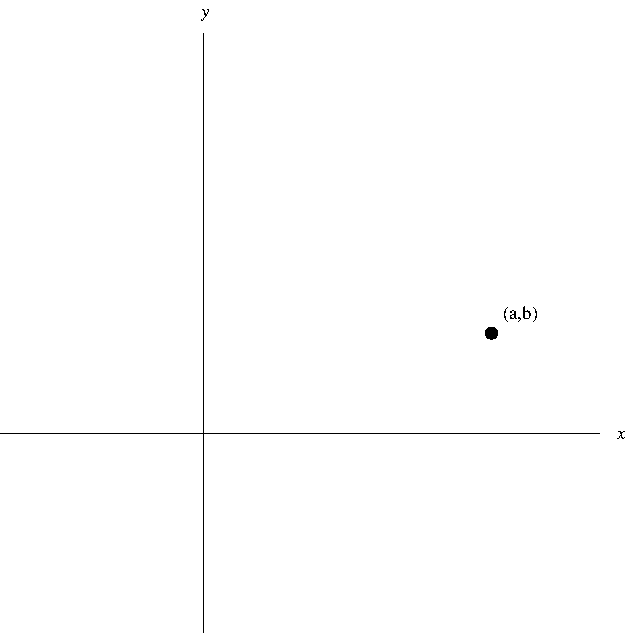
\includegraphics[height=4cm]{inverse-functions/pictures/07-01-reflecta.pdf}%
%}%
%\only<handout:0| 5>{%
%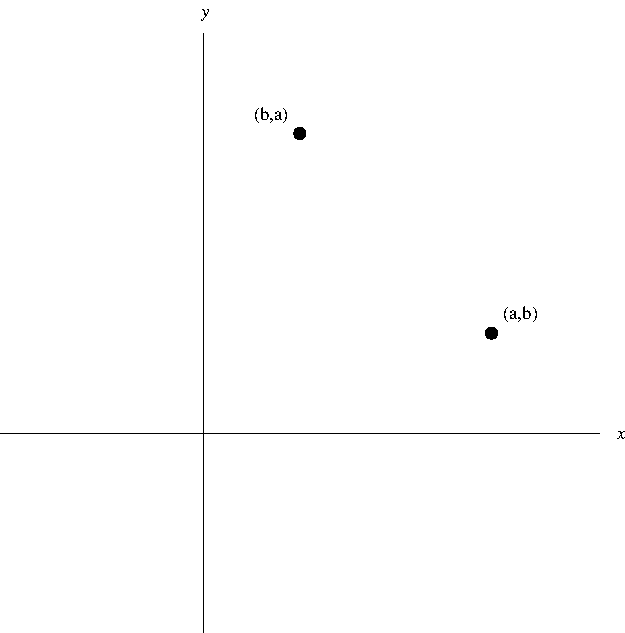
\includegraphics[height=4cm]{inverse-functions/pictures/07-01-reflectb.pdf}%
%}%
%\only<handout:1| 6->{%
%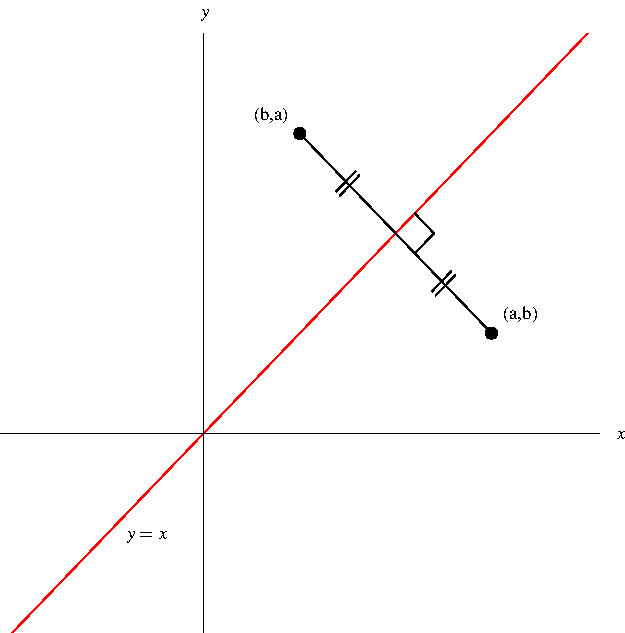
\includegraphics[height=4cm]{inverse-functions/pictures/07-01-reflectc.pdf}%
%}%
&%
\psset{xunit=1cm, yunit=1cm}
\begin{pspicture}(-5, -5)(5,5) 
\psframe*[linecolor=white](-5,-5)(5,5) 
\psaxes[ticks=none, labels=none]{<->}(0,0)(-1.5,-1.5)(3,3)
\psplot[linecolor=red, plotpoints=1000]{-0.292893219}{3}{x 1 add ln  0.693147181 div 1 sub}
\rput[lb](0.9, 2.4){\footnotesize $y=f^{-1}(x)$}
\uncover<7->{
%Function formula: 2^{1+x}-1 
\psplot[linecolor=red, plotpoints=1000]{-1.5}{0.95}{-1 2 x 1 add exp add }
\psline[linecolor=blue](-1.4, -1.4)(2.9,2.9)
\rput[l](-1, -1.2){\footnotesize $y=x$}
\rput[tr](2.8, 0.4){\footnotesize $y=f(x)$}
}
\end{pspicture} 
%\only<handout:0| -6>{%
%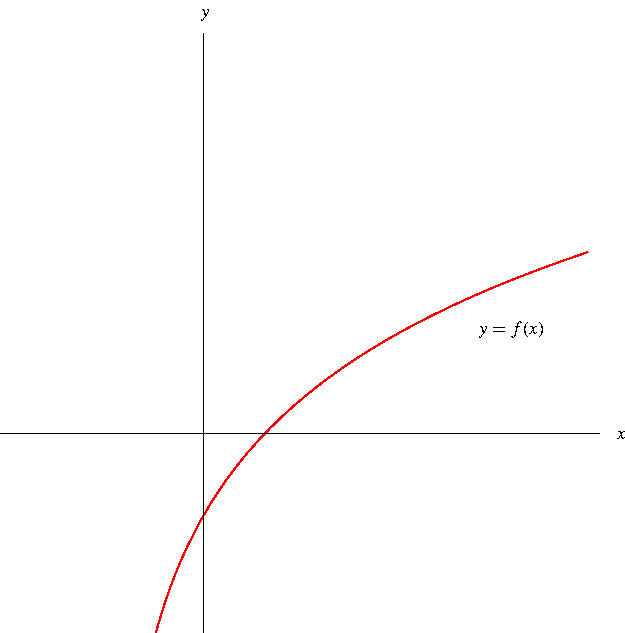
\includegraphics[height=4cm]{inverse-functions/pictures/07-01-reflect-functionb.pdf}%
%}%
%\only<handout:1| 7->{%
%\includegraphics[height=4cm]{inverse-functions/pictures/07-01-reflect-f unctiona.pdf}%
%}%
\end{tabular}

\footnotesize 
Interchanging $x$ and $y$ suggests a relation between the graphs of $f^{-1}$ and $f$:
\begin{itemize}
\item<2->  Suppose $(a,b)$ is on the graph of $f$.
\item<3->  Then $f(a) = b$.
\item<4->  Then $f^{-1}(b) = a$.
\item<5->  Then $(b,a)$ is on the graph of $f^{-1}$.
\item<6->  $(b,a)$ is the reflection of $(a,b)$ in the line $y = x$.
\item<7->  Therefore the graph of $f^{-1}$ is obtained by reflecting the graph of $f$ across the line $y = x$.
\end{itemize}
\end{frame}
% end module inverse-function-graph
